\chapter{Java静态安全扫描工具需求分析与设计}
\section{系统整体概述}
Java语言通常用于Web服务和Android程序开发,其中的大量安全漏洞类型可以通过污点传播分析法进行扫描,然而随着漏洞种类和开发方式不断丰富,污点分析存在失误,因此产生了大量误报,为此安全工程师不得不修改污点传播规则,以增加漏报为代价换取低误报,或是人工对大量误报漏洞判断,这两种做法无疑会增加潜在安全风险。

本系统旨在提供对于Java代码的更精确的漏洞静态扫描功能,在源代码开发阶段进行代码安全扫描。相对于传统污点传播扫描工具,本系统结合了程序切片和BLSTM,从已有的误报漏洞片段进行分析辅助污点传播,从而降低误报率。系统总体架构如图~\ref{overview}所示,系统主要分为前端和后端两大部分,前端部分运行在用户端,包含污点分析模块、程序切片模块、部分预测模块,而在扫描系统后端运行在服务器端,包含预处理模块,另一部分预测模块和数据库。

污点分析模块对开源的find-sec-bugs做改进,使之能够输出污点传播树,为误报预测提供基础数据;程序切片模块分析污点传播树,将其拆分为子污点传播流,利用Joana生成SDG并进行切片;数据预处理模块将切片模块的输出数据进行泛化和向量化处理,使之可以输出预测模块;误报预测模块利用切片模块的子污点传播流和其对应切片,通过BLSTM进行切片预测,从而对漏洞进行预测。本系统采用客户端采用Java进行开发,管理后台和程序预测服务由Python和Django开发。

\begin{figure}[htb]
	\centering
	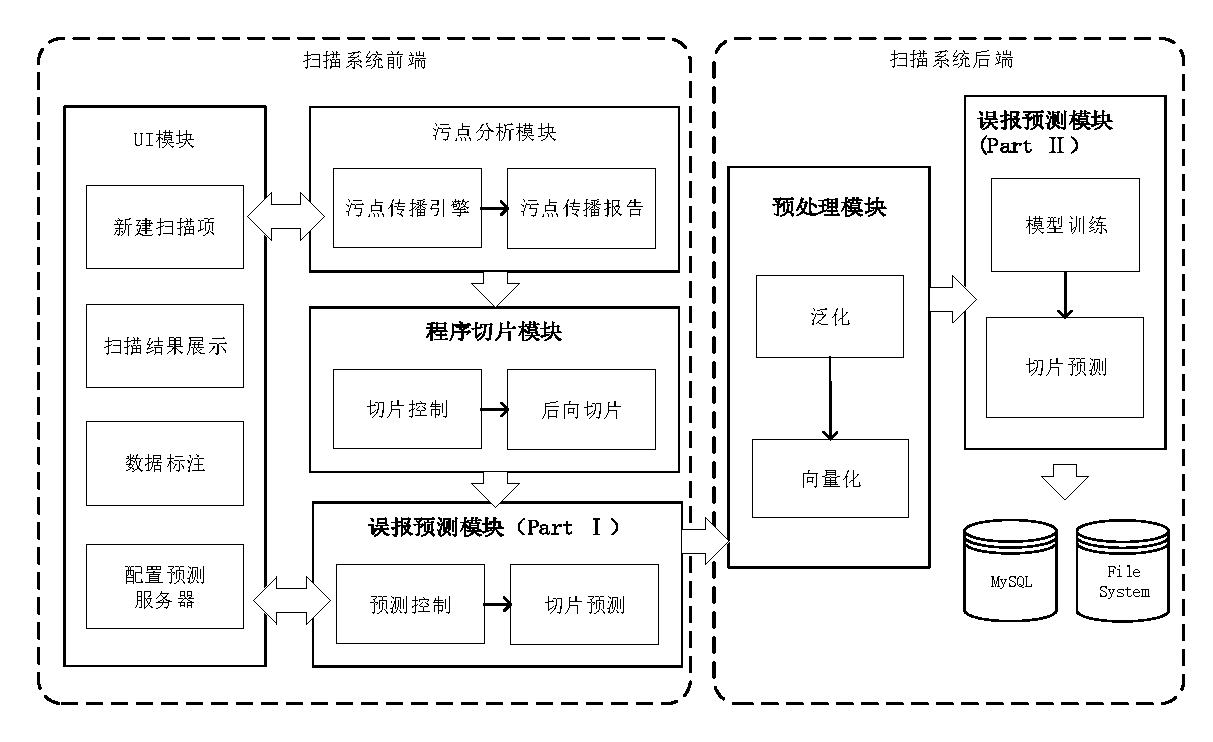
\includegraphics[width=5in]{FIGs/chapter3/system-architecture.pdf}
	\caption{系统总体架构图}\label{overview}
\end{figure}

\section{系统需求分析}
\subsection{功能性需求}
本系统功能性需求分析按污点分析模块,程序切片模块,预处理模块和误报预测模块四个方面进行。

污点分析模块由污点分析引擎对用户提交的jar文件进行扫描,产生初步结果,该模块所涉及的功能性需求如表~\ref{dmd:taint}所示,其主要功能为污点分析,而对于用户来说,系统需要友好的展现污点分析结果,即存在构造污点传播树和查看分析结果的需求,污点传播树由污点传播图构造而来,因此存在构造污点传播图需求,此外,污点分析是一项耗时操作,用户(尤其是开发工程师)可能会对一次污点分析结果进行保存,交给安全工程师进行漏洞验证,因此系统最好还需有保存分析结果和读取分析结果功能。
\begin{table}[!htbp]\footnotesize %label table
	\centering
	\caption{污点分析模块功能性需求列表}
	\vspace{2mm}
	% l - left, r - right, c - center. | means one vertical line 这里声明的是表格单元中的内容如何对齐
	\begin{tabular}{L{1.3cm}L{2.5cm}L{6.8cm}L{1.5cm}}
		\toprule
		\textbf{需求编号}&\textbf{需求名称}&\textbf{需求内容}&\textbf{优先级}\\
		\midrule
		R1	& 污点分析 				& 对于用户上传的代码进行污点分析,包括了过程内分析和过程间分析 & 高 \\
		R2  & 构造污点传播图 	 & 对于代码中存在的汇聚点,构造其污点传播图 & 高 \\
		R3  & 构造污点传播树	 & 对于一个污点传播类型的分析结果,用户最终看到一棵或多课污点传播树,其由污点传播图构造,一张污点传播图可能有多棵传播树,一个传播树上清晰标注有一个产生点和一或多个汇聚点 & 高 \\
		R4  & 查看分析结果	 & 对于一个污点传播类型的分析结果,用户最终看到一棵或多课污点传播树,对于树上的叶子节点,用户能够知晓其代码位置 & 高 \\
		R5  & 保存分析结果	   &用户可以对当前代码的漏洞分析详情进行保存,其中关键点在于对污点传播树进行序列化 & 中 \\
		R6  & 读取分析结果 	   &用户可以对保存后的分析结果文件进行读取,二次查看漏洞详情,其中关键点在于对污点传播树结构的反序列化 & 中 \\
		\bottomrule
	\end{tabular}
	\label{dmd:taint}
\end{table}

程序切片模块对污点分析结果进行切片处理,该模块所涉及的功能性需求如表~\ref{dmd:slice}所示,该模块的主要功能是根据污点分析模块的分析结果进行后向程序切片,将其拆解,得到四个子需求,首先其需要污点分析的结果进行处理,接着对污点传播树进行拆分,对于每一个污点传播流,其包含有若干个程序切片需求,下一步对这些需求进行后向切片,最后将切片结果转换为有一定结构的文本。

\begin{table}[!htbp]\footnotesize %label table
	\centering
	\caption{程序切片模块功能性需求列表}
	\vspace{2mm}
	% l - left, r - right, c - center. | means one vertical line 这里声明的是表格单元中的内容如何对齐
	\begin{tabular}{L{1.3cm}L{2.5cm}L{6.8cm}L{1.5cm}}
		\toprule
		\textbf{需求编号}&\textbf{需求名称}&\textbf{需求内容}&\textbf{优先级}\\
		\midrule
		R7	 & 处理污点分析结果 & 对污点分析的结果进行处理,对于每一个漏洞实例,反序列化的污点传播树并转化为适用于切片的传播树表达形式 & 高 \\
		R8	 & 污点传播树拆分 & 将每一个传播树拆分为一或多个污点传播流,每一个污点传播流包含若干个<函数入口点,关注点>对(其为一个切片的单位) & 高 \\
		R9   & 后向程序切片 & 对于每一个<函数入口点,关注点>, 结合用户上传的Jar包,进行后向程序切片 & 高 \\
		R10 & 输出切片结果	 & 对于切片,程序能将其表示为文本,即对切片结构体序列化 & 高 \\
		\bottomrule
	\end{tabular}
	\label{dmd:slice}
\end{table}

预处理模块对切片结果进行预处理,该模块所涉及的功能性需求如表~\ref{dmd:preprocessing}所示,该模块的主要功能是对切片文本进行泛化和向量化,在泛化需求主要保证一个切片能代表一类代码片段;随后进行向量化,对于切片的单词序列进行token标记,从而产生字典和切片向量,即BLSTM模型的输入。此外,一个较低优先级的需求为根据字典,将切片向量还原为切片的单词序列。

\begin{table}[!htbp]\footnotesize %label table
	\centering
	\caption{预处理模块功能性需求列表}
	\vspace{2mm}
	% l - left, r - right, c - center. | means one vertical line 这里声明的是表格单元中的内容如何对齐
	\begin{tabular}{L{1.3cm}L{2.5cm}L{6.8cm}L{1.5cm}}
		\toprule
		\textbf{需求编号}&\textbf{需求名称}&\textbf{需求内容}&\textbf{优先级}\\
		\midrule
		R11   & 泛化 & 对于每一个切片进行泛化处理,包括抽象数值、字符串、类名和方法名等 & 高 \\
		R12 & 向量化	 & 对于一个切片的单词序列,生成单词与整形值的字典并按字典对其向量化 & 高 \\
		R13 & 反向量化	 & 对于一个单词序列的向量,根据字典将其还原为切片的单词序列 & 低 \\
		\bottomrule
	\end{tabular}
	\label{dmd:preprocessing}
\end{table}

误报预测模块是对保障漏洞报告准确性的核心模块,包括客户端、后端和Web前端部分,该模块所涉及的功能性需求如表~\ref{dmd:predict}所示,该模块的需求主要为对给定漏洞实例进行预测,标记以及模型训练。预测依赖后端服务,因此有设置后端服务器的需求;预测分为预测切片安全性需求和预测漏洞真实性需求,分别由后端服务和客户端实现;标记分为对切片安全性标记和漏洞真实性标记,当漏洞标记为误报时,用户需指定安全的污染流;同时,管理员有训练预测模型的需求;此外,由于预测过程并不是很占用资源,对保存预测结果的需求程度较低;最后用户可以清空标记和预测结果。

\begin{table}[!htbp]\footnotesize %label table
	\centering
	\caption{误报预测模块功能性需求列表}
	\vspace{2mm}
	% l - left, r - right, c - center. | means one vertical line 这里声明的是表格单元中的内容如何对齐
	\begin{tabular}{L{1.3cm}L{2.5cm}L{6.8cm}L{1.5cm}}
		\toprule
		\textbf{需求编号}&\textbf{需求名称}&\textbf{需求内容}&\textbf{优先级}\\
		\midrule
		R14 & 预测切片安全性 & 对于一个切片向量,预测该切片是否是安全的(污染流无法传播) & 高 \\
		R15 & 标记切片安全性	 & 对切片向量,标记其是否安全 & 高 \\
		R16 & 预测漏洞真实性 & 用户在客户端可以查看预测结果,即该漏洞是否真实存在,需要结合切片预测需求 & 高 \\
		R17 & 标记漏洞真实性	 & 用户在客户端可以对于一个漏洞,标记漏洞是否存在,不存在时用户需提供理由(指出安全的污染流) & 高 \\
		R18 & 训练预测模型	 & 管理员可以在Web页面发起训练模型任务,或是安排定时器定期更新模型 & 高 \\
		R19 & 保存预测结果	 & 用户在客户端可以保存漏洞预测结果 & 低 \\
		R20 & 清空标记和预测结果	 & 用户在客户端可以清空标记和预测结果,以便重新预测 & 低 \\
		R21 & 设置预测服务器	 & 用户在客户端设置远程服务器 & 中 \\
		\bottomrule
	\end{tabular}
	\label{dmd:predict}
\end{table}


\subsection{非功能性需求}
本系统旨在为开发者和安全工程师提供Java代码安全扫描功能,考虑到系统功能性质、使用场景和所属领域,系统的非功能性需求主要有高效率,健壮性,保密性,安全性和扩展性五点。

首先,本系统的功能点在于对Java代码进行安全扫描,其使用场景位于软件开发至测试阶段,因此扫描过程要保证一定的效率和健壮性,如果一次扫描等待时间过长,或是扫描过程中途崩溃,那么开发过程就会受到影响,甚至影响整个服务的可用性,因此本系统需要是高效且健壮的。

其次,本系统涉及软件安全领域,很可能是恶意攻击者的首要攻击对象,因此自身需要具备保密性和安全性,这里的保密性是指保证用户提交的Java代码和Jar包的数据安全,安全性是指扫描服务本身经过充分安全性测试,不出现安全漏洞。

最后,很多企业目前已经拥有了适用于自身特点的基于污点传播的扫描器,为此,系统需要保证一定的扩展性,如将污点传播的解析抽象为接口,保证其可以基于任意污点传播工具进行预测。\\

\subsection{系统用例描述}
%用例图
本系统的主要用户为软件开发工程师和软件安全运营人员,根据对系统需求的分析,得到系统用例如图~\ref{fig:case}所示, 软件开发工程师和运营人员均有基于污点分析的静态扫描、扫描结果切片和预测、漏洞实例标记这三个用例,其中基于污点分析的静态扫描存在两例扩展用例,即保存污点分析结果和读取分析结果,漏洞实例标记实际包含了标记正报结果和标记误报结果用例,安全运营人员还多出模型训练和发放客户端口令的用例。

\begin{figure}[!htbp]
	\centering
	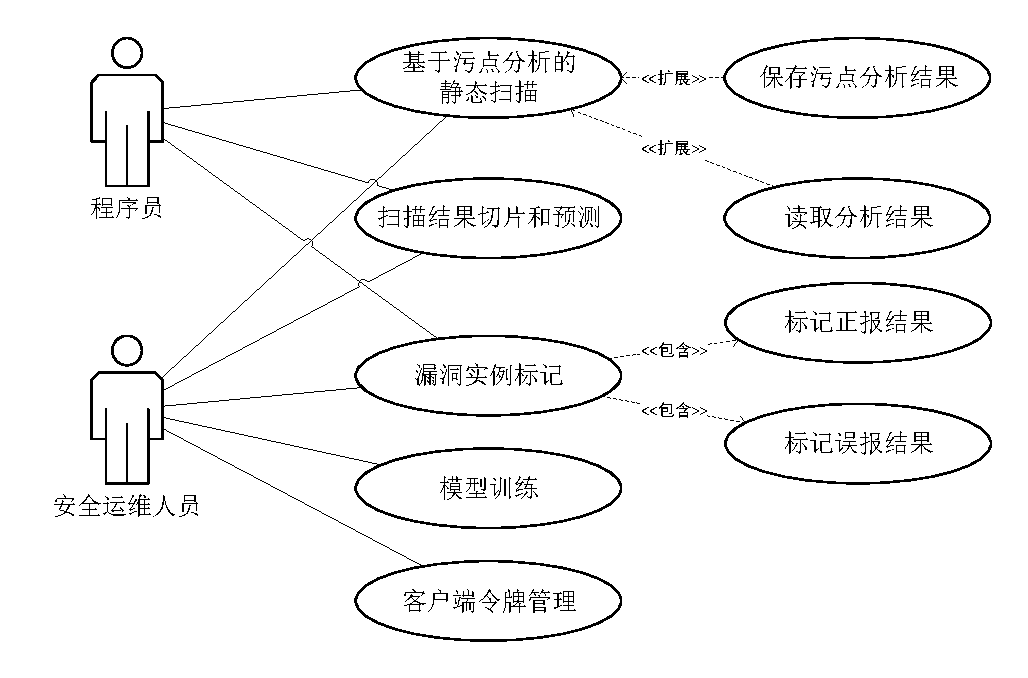
\includegraphics[width=5in]{FIGs/chapter3/case.pdf}
	\caption{系统用例图}\label{fig:case}
\end{figure}

\newcounter{caseCounter}
\setcounter{caseCounter}{1}

基于污点分析进行程序的静态扫描是本系统的基本功能,同样也是漏洞预测的基础。其用例描述如表~\ref{case:taint}所示,安全工程师或软件工程师(下面统称“用户”)对将开发好的项目进行构建,新建项目时将源代码和构建得到的Jar/War包添加到项目中,随后系统对其进行污点分析,并返回给用户潜在的安全漏洞。
% 1基于污点分析的静态扫描
\begin{table}[!htb]\footnotesize %label table
	\centering
	\caption{基于污点分析的静态扫描用例描述}
	\vspace{2mm}
	% l - left, r - right, c - center. | means one vertical line 这里声明的是表格单元中的内容如何对齐
	\begin{tabular}{L{3cm}L{10cm}}
		\toprule
		\textbf{描述项}&\textbf{说明}\\
		\midrule
		用例编号 & C\arabic{caseCounter}\stepcounter{caseCounter} \\
		用例名称 & 基于污点分析的静态扫描用例 \\
		对应功能需求编号  & R1, R2, R3, R4 \\ 
		参与者 & 用户 \\
		前置条件 & 用户已开发好项目并已构建的Jar/War包 \\
		后置条件 & 无\\
		正常流程 & \tabincell{l}{
							1. 用户选择“文件”,“新建项目”,打开新建项目会话框\\
							2. 用户输入项目名称,选择需要分析的包文件以及源文件所在目录\\
							3. 用户点击“分析”按钮,程序开始对其进行基于污点分析的静态扫描\\
							4. 用户在界面上看到漏洞列表,点击一个污点传播类型的漏洞\\
							5. 用户在界面上看到该漏洞的污点传播树\\
							6. 用户点击任意污点传播树的叶子节点,在界面上看到对应的源代码
					}\\
		异常流程 & 2. 若出现异常,则弹出异常会话框并显示异常信息\\
		\bottomrule
	\end{tabular}
	\label{case:taint}
\end{table}

% 2保存分析结果
污点分析后,用户可以对其分析结果进行保存,其用例描述见表~\ref{case:taintsave},用户点击保存按钮后,系统将污点传播树的每一节点序列化漏洞注解,并将含有一组注解的一系列漏洞保存为本地文件。

\begin{table}[!htb]\footnotesize %label table
	\centering
	\caption{保存污点分析结果用例描述}
	\vspace{2mm}
	% l - left, r - right, c - center. | means one vertical line 这里声明的是表格单元中的内容如何对齐
	\begin{tabular}{L{3cm}L{10cm}}
		\toprule
		\textbf{描述项}&\textbf{说明}\\
		\midrule
		用例编号 & C\arabic{caseCounter}\stepcounter{caseCounter}  \\
		用例名称 & 保存污点分析结果用例 \\
		对应功能需求编号  & R5 \\ 
		参与者 & 用户  \\
		前置条件 & 用户已创建项目且进行了基于污点分析的静态扫描 \\
		后置条件 & 用户指定位置出现保存好的分析报告\\
		正常流程 & \tabincell{l}{
			1. 用户选择“文件”,“另存为”,打开另存为对话框\\
			2. 用户输入保存文件名、文件类型和保存位置,点击保存按钮,分析结果\\被保存
		}\\
		异常流程 & 2. 若出现异常,则弹出异常会话框并显示异常信息\\
		\bottomrule
	\end{tabular}
	\label{case:taintsave}
\end{table}

% 3读取分析结果
对于以保存的分析结果,用户可以加载它们重新分析漏洞结果,程序对分析结果反序列化后在界面显示先前分析结果,如表~\ref{case:taintload}所示。

\begin{table}[!htb]\footnotesize %label table
	\centering
	\caption{读取分析结果用例描述}
	\vspace{2mm}
	% l - left, r - right, c - center. | means one vertical line 这里声明的是表格单元中的内容如何对齐
	\begin{tabular}{L{3cm}L{10cm}}
		\toprule
		\textbf{描述项}&\textbf{说明}\\
		\midrule
		用例编号 & C\arabic{caseCounter}\stepcounter{caseCounter}  \\
		用例名称 & 读取分析结果用例 \\
		对应功能需求编号  & R6 \\ 
		参与者 & 用户  \\
		前置条件 & 用户磁盘中已有一份污点分析报告 \\
		后置条件 & 无\\
		正常流程 & \tabincell{l}{
			1. 用户选择“文件”,“打开”,显示打开文件对话框\\
			2. 用户在打开文件对话框中选择报告文件,点击“打开”按钮,程序\\加载并在界面上显示污点分析报告中的内容
		}\\
		异常流程 & 2. 若出现异常,则弹出异常会话框并显示异常信息息\\
		\bottomrule
	\end{tabular}
	\label{case:taintload}
\end{table}

% 4设置预测服务器
对于客户端来说,对漏洞进行标记或者预测前提需要设置远程服务器,设置预测服务器的用例描述如表~\ref{case:setserver}所示,用户通过管理员发放的token和服务器地址设置远端服务器。
\begin{table}[!htb]\footnotesize %label table
	\centering
	\caption{设置预测服务器用例描述}
	\vspace{2mm}
	% l - left, r - right, c - center. | means one vertical line 这里声明的是表格单元中的内容如何对齐
	\begin{tabular}{L{3cm}L{10cm}}
		\toprule
		\textbf{描述项}&\textbf{说明}\\
		\midrule
		用例编号 & C\arabic{caseCounter}\stepcounter{caseCounter}  \\
		用例名称 & 设置预测服务器用例 \\
		对应功能需求编号  & R21 \\ 
		参与者 & 用户  \\
		前置条件 & 管理员已向用户发放token \\
		后置条件 & 无\\
		正常流程 & \tabincell{l}{
			1. 用户选择“AI”,“Set Server”,显示服务器设置对话框\\
			2. 用户服务器对话框汇中设置服务器地址以及token信息\\
			3. 用户点击“验证”按钮,检查配置是否正确\\
			4. 用户点击“应用”按钮,完成服务器配置
		}\\
		异常流程 & 2. 若出现异常,则弹出异常会话框并显示异常信息\\
		\bottomrule
	\end{tabular}
	\label{case:setserver}
\end{table}

% 5扫描结果预测
扫描结果切片和预测功能是本系统的最核心功能,程序首先对污点传播结果分析,拆解为污点传播片段并分别切片,再由服务端预测每一个切片是否为清洁片段,最后得出漏洞实例是否为真实漏洞。涉及的用例描述如表~\ref{case:predict}所示。

\begin{table}[!htbp]\footnotesize %label table
	\centering
	\caption{扫描结果切片和预测用例描述}
	\vspace{2mm}
	% l - left, r - right, c - center. | means one vertical line 这里声明的是表格单元中的内容如何对齐
	\begin{tabular}{L{3cm}L{10cm}}
		\toprule
		\textbf{描述项}&\textbf{说明}\\
		\midrule
		用例编号 & C\arabic{caseCounter}\stepcounter{caseCounter}  \\
		用例名称 & 扫描结果切片和预测用例 \\
		对应功能需求编号  & R7, R8, R9, R10, R14, R16 \\ 
		参与者 & 用户  \\
		前置条件 & 用户已完成远程服务器配置并且已有污点分析结果 \\
		后置条件 & 预测所需所有切片信息发送至服务器\\
		正常流程 & \tabincell{l}{
			1. 用户选择“AI”点击“Slice and Predict”,程序开始对污点分析结\\果进行切片和预测\\
			2. 用户等待切片和预测完成时,可以在弹出的会话框中观察预测进度,\\并随时取消预测\\
			3. 用户在程序主界面看到每一漏洞预测结果,预测为误报的漏洞由灰色\\图标标识且在漏洞列表标注为“(P: FP)”,预测结果为正报的漏洞图标\\不变,文字标注为“(P: TP)”\\
			4. 用户在点击一个漏洞,在污点传播图上可以看到预测解释,当预测结果\\为误报时,所有与预测为安全的污点传播流相关的叶子节点由“(*)”标\\注。
		}\\
		异常流程 & 2. 若出现异常,则弹出异常会话框并显示异常信息\\
		\bottomrule
	\end{tabular}
	\label{case:predict}
\end{table}

% 6标记正报结果
若漏洞实例被安全工程师判断为真实存在的,工程师可以对该漏洞标记为正报,此时所有污染流片段均自动标记为不安全,并且发送给服务端。标记正报结果用例描述如表~\ref{case:labeltp}所示。

\begin{table}[!htbp]\footnotesize %label table
	\centering
	\caption{标记正报结果用例描述}
	\vspace{2mm}
	% l - left, r - right, c - center. | means one vertical line 这里声明的是表格单元中的内容如何对齐
	\begin{tabular}{L{3cm}L{10cm}}
		\toprule
		\textbf{描述项}&\textbf{说明}\\
		\midrule
		用例编号 & C\arabic{caseCounter}\stepcounter{caseCounter}  \\
		用例名称 & 标记正报结果用例 \\
		对应功能需求编号  & R15, R17 \\ 
		参与者 & 用户  \\
		前置条件 & 用户已经对污点分析结果进行了切片和预测 \\
		后置条件 & 用户指定漏洞的所有污染流片段均标记为不安全且发送至服务器\\
		正常流程 & \tabincell{l}{
			1. 用户右键点击需要标记的正报漏洞实例,弹出标记菜单\\
			2. 用户点击“Labeled as True Positive”,该漏洞被标记为正报,漏洞说\\明内容被显示为“[L: TP]”
		}\\
		异常流程 & 2. 若出现异常,则弹出异常会话框并显示异常信息\\
		\bottomrule
	\end{tabular}
	\label{case:labeltp}
\end{table}

% 7标记误报结果
若漏洞实例被用户判断为不存在,用户可以对该漏洞标记为误报,此时用户需要指定一条最短的污染流,并且在该污染流中污点消失,同时,这段“安全的污染流”被发送至服务端。标记误报结果用例描述如表~\ref{case:labelfp}所示。

\begin{table}[!htb]\footnotesize %label table
	\centering
	\caption{标记误报结果用例描述}
	\vspace{2mm}
	% l - left, r - right, c - center. | means one vertical line 这里声明的是表格单元中的内容如何对齐
	\begin{tabular}{L{3cm}L{10cm}}
		\toprule
		\textbf{描述项}&\textbf{说明}\\
		\midrule
		用例编号 & C\arabic{caseCounter}\stepcounter{caseCounter}  \\
		用例名称 & 标记误报结果用例 \\
		对应功能需求编号  &  R15, R17 \\ 
		参与者 & 用户  \\
		前置条件 & 用户已经对污点分析结果进行了切片、预测或标记 \\
		后置条件 & 无\\
		正常流程 & \tabincell{l}{
			1. 用户右键点击需要标记的误报漏洞实例,弹出标记菜单\\
			2. 用户点击“Labeled Safe Flow”,弹出误报标记会话框\\
			3. 用户选择一条最短的安全污染流,同时看到该污染流的哈希和切片信\\息,点击确定后完成标记\\
			4. 用户看到其所标记的漏洞被标注为“[L: FP]”,并且在污染传播树中,\\所有与被用户标记的那段污染流相关的叶子节点由“[*]”标记。
		}\\
		异常流程 & 2. 若出现异常,则弹出异常会话框并显示异常信息\\
		\bottomrule
	\end{tabular}
	\label{case:labelfp}
\end{table}

% 8清空切片、标记和预测结果
由于切片、预测是复杂操作,系统会将其放入缓存,同时标记结果用户也会有想清空的情况,因此本系统提供一键清除切片、标记和预测结果的功能。其用例描述如表~\ref{case:clean}所示。
\begin{table}[!htb]\footnotesize %label table
	\centering
	\caption{清空切片、标记和预测结果用例描述}
	\vspace{2mm}
	% l - left, r - right, c - center. | means one vertical line 这里声明的是表格单元中的内容如何对齐
	\begin{tabular}{L{3cm}L{10cm}}
		\toprule
		\textbf{描述项}&\textbf{说明}\\
		\midrule
		用例编号 & C\arabic{caseCounter}\stepcounter{caseCounter}  \\
		用例名称 & 清空切片、标记和预测结果用例 \\
		对应功能需求编号  & R20 \\ 
		参与者 & 用户  \\
				前置条件 & 用户已经对污点分析结果进行了切片和预测 \\
		后置条件 & 用户指定漏洞的最短安全污染流被标记为安全且发送至服务器\\
		正常流程 & \tabincell{l}{
			1. 用户选择“AI”点击“Clean DB”,程序清空切片、预测和标记数据,\\并在漏洞的预测标签上显示“(P: UNK)”,在标记标签上显示“[L: UNK]”
		}\\
		异常流程 & 无\\
		\bottomrule
	\end{tabular}
	\label{case:clean}
\end{table}

% 9模型训练
模型训练的用例描述如表~\ref{case:train}所示,管理员通过在Web后端发起模型训练请求,系统会进行异步调用,通过消息队列,训练程序会根据选择的训练配置进行模型训练,并将训练模型保存,供预测时调用,用户也可以设置定时任务,是系统按时自动训练模型。
\begin{table}[!htb]\footnotesize %label table
	\centering
	\caption{模型训练用例描述}
	\vspace{2mm}
	% l - left, r - right, c - center. | means one vertical line 这里声明的是表格单元中的内容如何对齐
	\begin{tabular}{L{3cm}L{10cm}}
		\toprule
		\textbf{描述项}&\textbf{说明}\\
		\midrule
		用例编号 & C\arabic{caseCounter}\stepcounter{caseCounter}  \\
		用例名称 & 模型训练用例 \\
		对应功能需求编号  & R11, R12, R18 \\ 
		参与者 & 用户(这里特指安全运营人员)  \\
		前置条件 & 数据库中已存在用于训练的切片和标记数据 \\
		后置条件 & 数据库中记录已经训练好的模型\\
		正常流程 & \tabincell{l}{
			1. 用户登录 Web 控制台\\
			2. 用户在控制台中点击“Model Config”进入模型配置页面,查看或新\\建模型配置\\
			3. 用户在控制台中点击“Periodic Tasks”,进入任务页面,在任务页面\\
			中选择模型训练任务,并设置任务类型(定时任务或单次执行任务)并\\且指定时间,以及训练指定的模型配置,系统到规定时间后自动训练模\\型
		}\\
		异常流程 & \tabincell{l}{4. 若模型训练中遇到错误,将错误信息返回到任务结果表中,\\供用户查看}\\
		\bottomrule
	\end{tabular}
	\label{case:train}
\end{table}

客户端令牌管理的用例描述如表~\ref{case:train}所示,管理员通过在Web后端对客户端令牌进行管理,即对其进行增删改查操作。
\begin{table}[!htb]\footnotesize %label table
	\centering
	\caption{客户端令牌管理用例描述}
	\vspace{2mm}
	% l - left, r - right, c - center. | means one vertical line 这里声明的是表格单元中的内容如何对齐
	\begin{tabular}{L{3cm}L{10cm}}
		\toprule
		\textbf{描述项}&\textbf{说明}\\
		\midrule
		用例编号 & C\arabic{caseCounter}\stepcounter{caseCounter}  \\
		用例名称 & 客户端令牌管理用例 \\
		对应功能需求编号  & R21 \\ 
		参与者 & 安全运营人员  \\
		前置条件 & 无 \\
		后置条件 & 无 \\
		正常流程 & \tabincell{l}{
			1. 用户登录 Web 控制台\\
			2. 用户在控制台中点击“Client Token”进入客户端令牌管理页面,对客\\户端令牌进行增加,修改,删除等操作。
		}\\
		异常流程 & 无 \\
		\bottomrule
	\end{tabular}
	\label{case:token}
\end{table}

\section{系统总体设计}
本系统的框架图已在本节第一章图~\ref{overview}展示,下面将对系统设计的模块从逻辑视图、开发视图、进程视图、物理视图和场景视图五个方面详细介绍系统总体设计。% The 4+1 View Model of Architecture,Philippe Kruchten 

首先是逻辑视图,该视图主要反应本系统的对象设计,如图~\ref{logicview}所示,图中 AbstractTaintDetector 是污点传播分析类的抽象类,与之相关的类有MethodDescriptor 和 Location ,其分别表示函数摘要和代码位置;
AbstractIncjectionDetector 是注入类型漏洞分析器的抽象类,继承自 AbstractTaintDetector,相对于 AbstractTaintDetector 其主要增加了具有输出漏洞报告的功能,目前几乎所有污点传播漏洞类都继承该类;
与 AbstractIncjectionDetector 相关的有 InjectionSink 类,该类表示污点汇聚点,其记录汇聚点可产生污点传播图,即 TaintFlowGraph 类;
与 TaintFlowGraph 相关的有 TaintTreeGenerator ,即污点传播树生成类,其用于生成污点传播树,树上节点为 TaintTreeNode 类;
BugAnnotationWithSourceLines 是漏洞注解类,用于在用户界面上显示一个污点传播树的叶子节点;
若干棵污点传播树共同构成了一个漏洞实例——BugInstance类;若干个BugInstance类组合产生BugCollection,即一个项目的漏洞集合类;
SliceRunner 为切片控制类,其首先调用报告翻译器对漏洞报告进行翻译,产生污点项目类——TaintProject,接着调用切片器对程序进行切片,最终产生切片项目类——SliceProject;ReportParser 和 Slicer分别为翻译器和切片器的接口;
SpotbugsReportParser 为 Spotbugs 的报告翻译器,实现了翻译器接口,负责筛选find-sec-bugs的污点传播类型漏洞并进行翻译;
JoanaSlicer 为基于 Joana 的切片器,实现切片器接口;
切片项目中包含切片的集合,切片类为 Slice;
PredictRunner 为预测控制类其依赖预测器接口——Predictor 对漏洞实例进行预测,返回为预测项目类——PredictProject 的实例;
BLSTMRemotePredictor 为远程调用服务端预测接口的预测器,实现 Predictor 接口;
后端服务器的所有服务表示为 Service 类,其中包含对 BLSTM 模型的控制类 ModelController;
表示预处理的类有 Preprocessing 类,该类中有对切片的各类泛化操作,以及 Tokenizer 类,其中包含对切片的向量化和反向量化操作;
最后模型类表示为 BLSTM 类;其通过数据集 Dataset 类进行训练。

\begin{figure}[!htb]
	\centering
	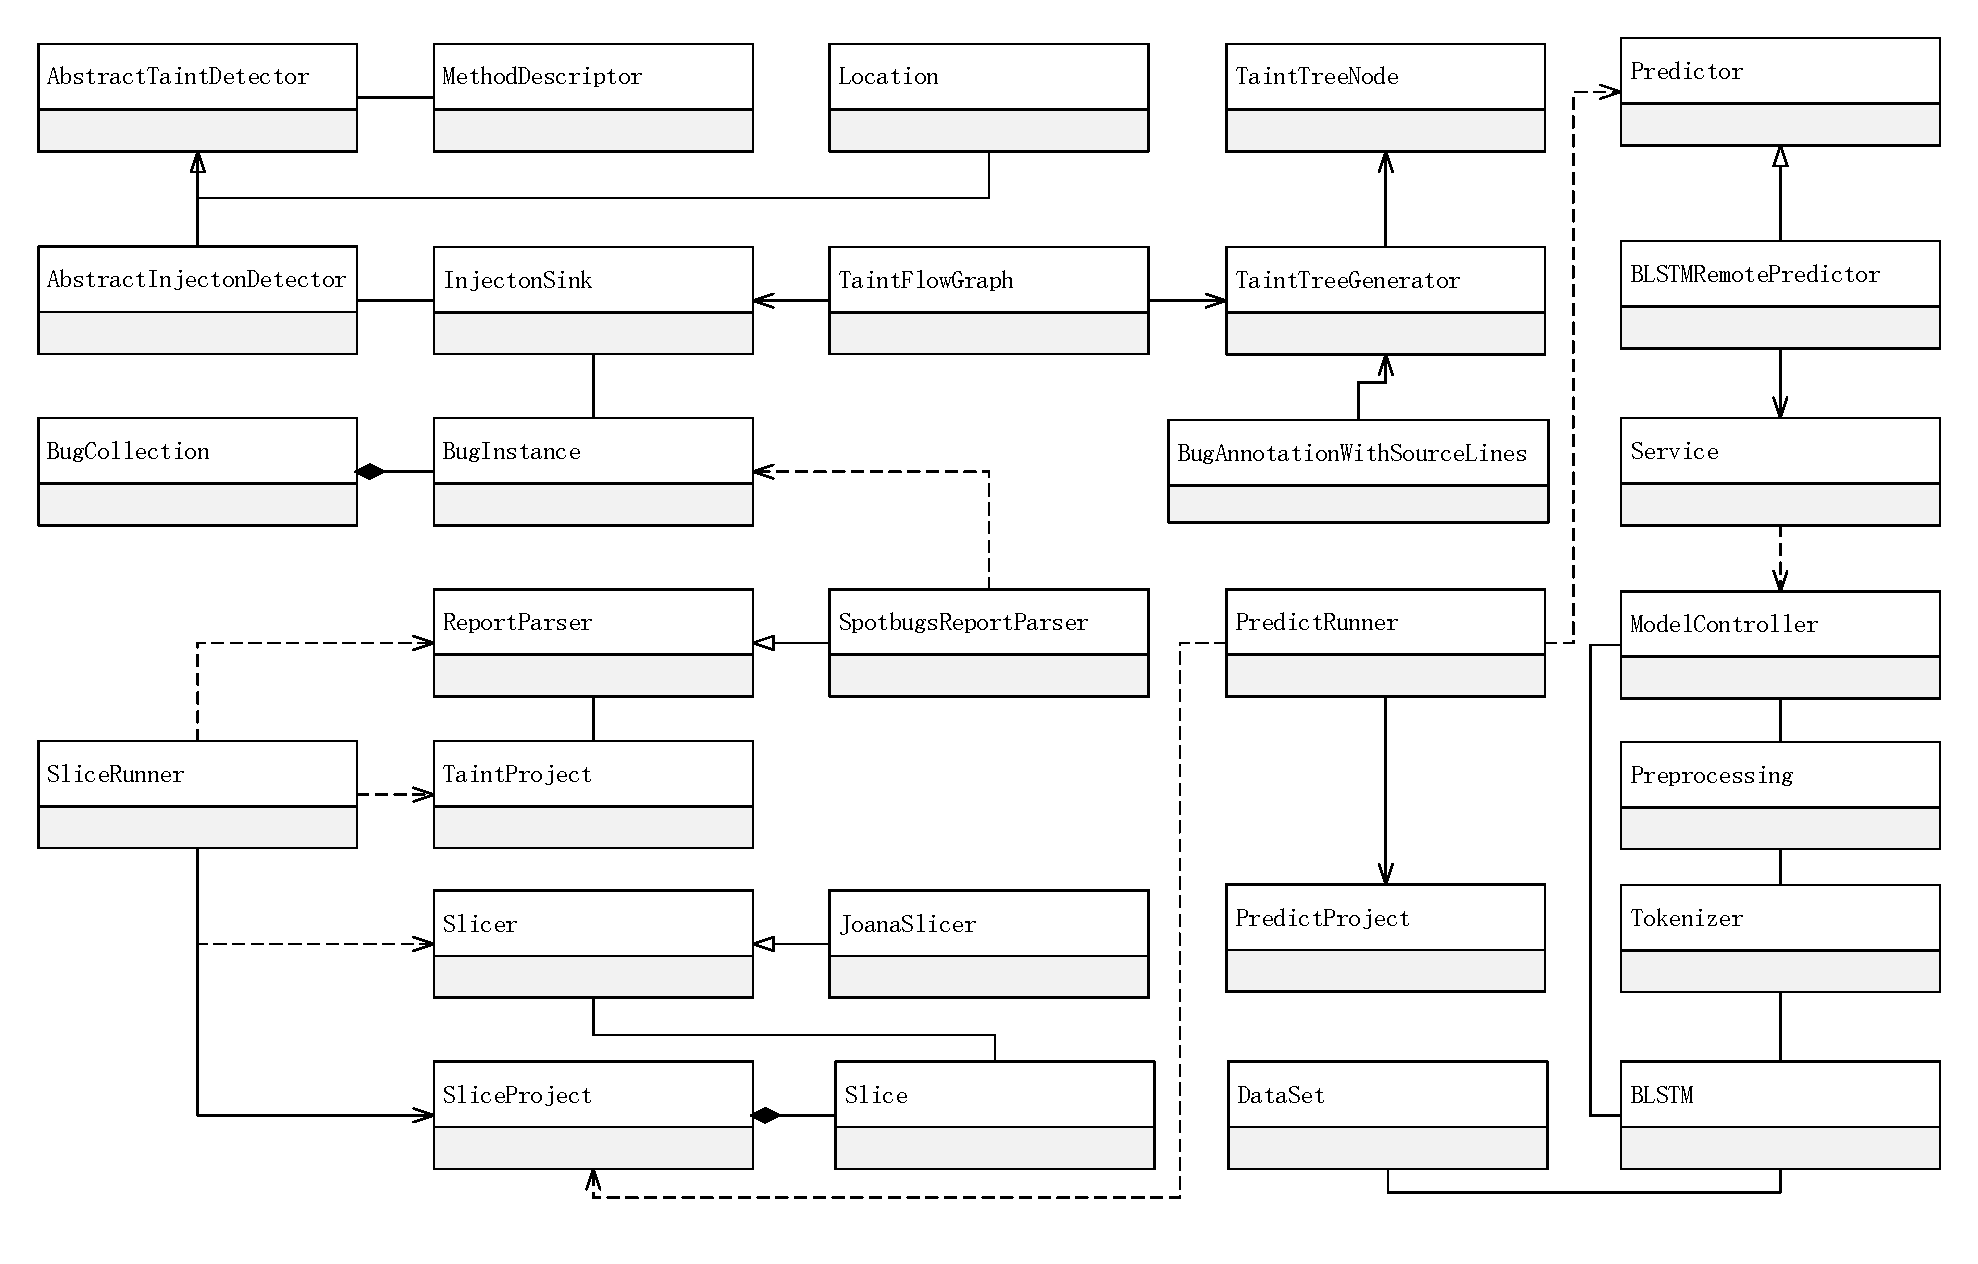
\includegraphics[width=5in]{FIGs/chapter3/logicview.pdf}
	\caption{系统逻辑视图}\label{logicview}
\end{figure}

% 逻辑视图=UML类图
% 开发视图=开发者角度,模块框图,加切片、预测模型
% 进程视图?
% 部署图,组件图

% 场景视图=用例图

\section{污点分析模块设计}
\subsection{类图设计}
函数调用图数据结构:

污染传播树数据结构:

\subsection{流程设计}

\section{程序切片模块设计}
\subsection{类图设计}
\subsection{流程设计}

\section{数据预处理模块设计}
\subsection{类图设计}
\subsection{流程设计}

\section{误报预测模块设计}
\subsection{架构设计}
\subsection{类图设计}
\subsection{流程设计}

\section{数据库设计}
本系统的数据库主要用来存储用户身份信息、污点分析得到的污染流数据和标记、用于模型训练的参数配置信息以及模型本身信息。经过分类,可以总结为三类数据表:

第一类是与鉴权有关的数据表,由于本系统主要使用了C/S架构,为了防止恶意攻击者向服务器注入垃圾数据影响预测,因此需要对客户端身份进行鉴定,为此设立客户端口令(Client\_Token)表,由安全运营人员进行维护。

第二类是与程序分析相关的数据表,由于本系统后台主要是对子污染流的切片进行有监督预测,因此自然需要污染流(Taint\_Flow)表和对污染流的标记(Label)表,对一个污染流而言,需要对其函数入口和关注点(即语句位置)进行切片,因此存在函数摘要(Method\_Description)表和语句位置(Location)表,不同项目可能具有名称相同的类、函数或文件,为了在逻辑上唯一标识一个函数摘要和语句位置,因此建立项目(Project)表。

第三类是与模型本身相关的数据表,本系统使用BLSTM进行切片预测,对BLSTM训练和BLSTM结构本身涉及到一系列参数,为此将其保存在模型配置(Model\_Config)表中,供安全运营人员调整,对于已经训练好的模型,将其保存在BLSTM模型(LSTM\_Model)表中。

与鉴权有关的数据表实体关系图如图~\ref{er:token} 所示,其中只有一张表,即客户端口令表,其中字段如表~\ref{sql:tokenTable} 所示,id 为一个口令的唯一标识;token 为一字符串,由管理员设置和发放,客户端连接时需要有一合法 token 才可与服务器通信;description 用于保存该口令的一些描述信息;create\_time 为该口令的创建时间。
\begin{figure}[!htbp]
	\centering
	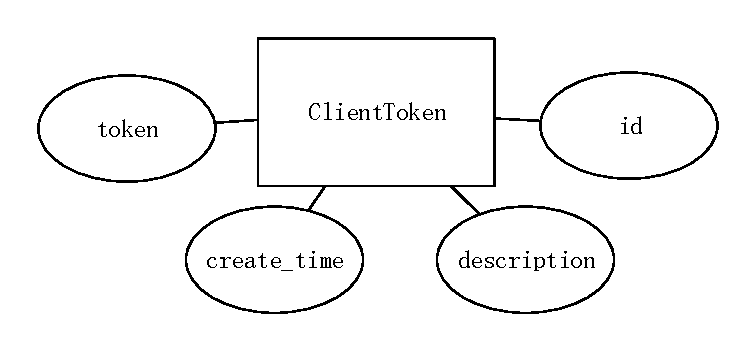
\includegraphics[width=0.5\linewidth]{FIGs/chapter3/token_er.pdf}
	\caption{与鉴权相关表的实体关系图}\label{er:token}
\end{figure}

\begin{table}[!htbp]\footnotesize %token table
	\centering
	\caption{Client\_Token 表}
	\vspace{2mm}
	% l - left, r - right, c - center. | means one vertical line 这里声明的是表格单元中的内容如何对齐
	\begin{tabular}{L{2cm}L{2cm}L{2.6cm}L{6cm}}
		\toprule
		\textbf{字段名}&\textbf{数据类型}&\textbf{属性}&\textbf{说明}\\
		\midrule
		id					&INT&PK&主键,token的唯一标识\\
		token 				&VARCHAR(255)&NN, UNIQUE&表示管理员向用户发放的 token\\
		description				 &VARCHAR(255)& N &用于保存管理员对此 token 的备注信息\\
		create\_time		  &DATETIME&NN&表示 token 的创建时间\\
		\bottomrule
	\end{tabular}
	\label{sql:tokenTable}
\end{table}

与程序分析相关的实体关系图如图~\ref{er:program},其中,项目表保存项目名称,函数摘要表保存一个项目中的函数摘要信息,语句位置表记录关注点所在的代码位置,污染流表记录污染流和其中的切片信息,标记表记录一个污染流记录是否是安全的。一个项目可以有多个函数摘要、位置和污染流,即有一对多的关系,一个函数摘要或语句位置可以有多个污染流记录,而标记和污染流记录呈一对一关系。

\begin{figure}[!htbp]
	\centering
	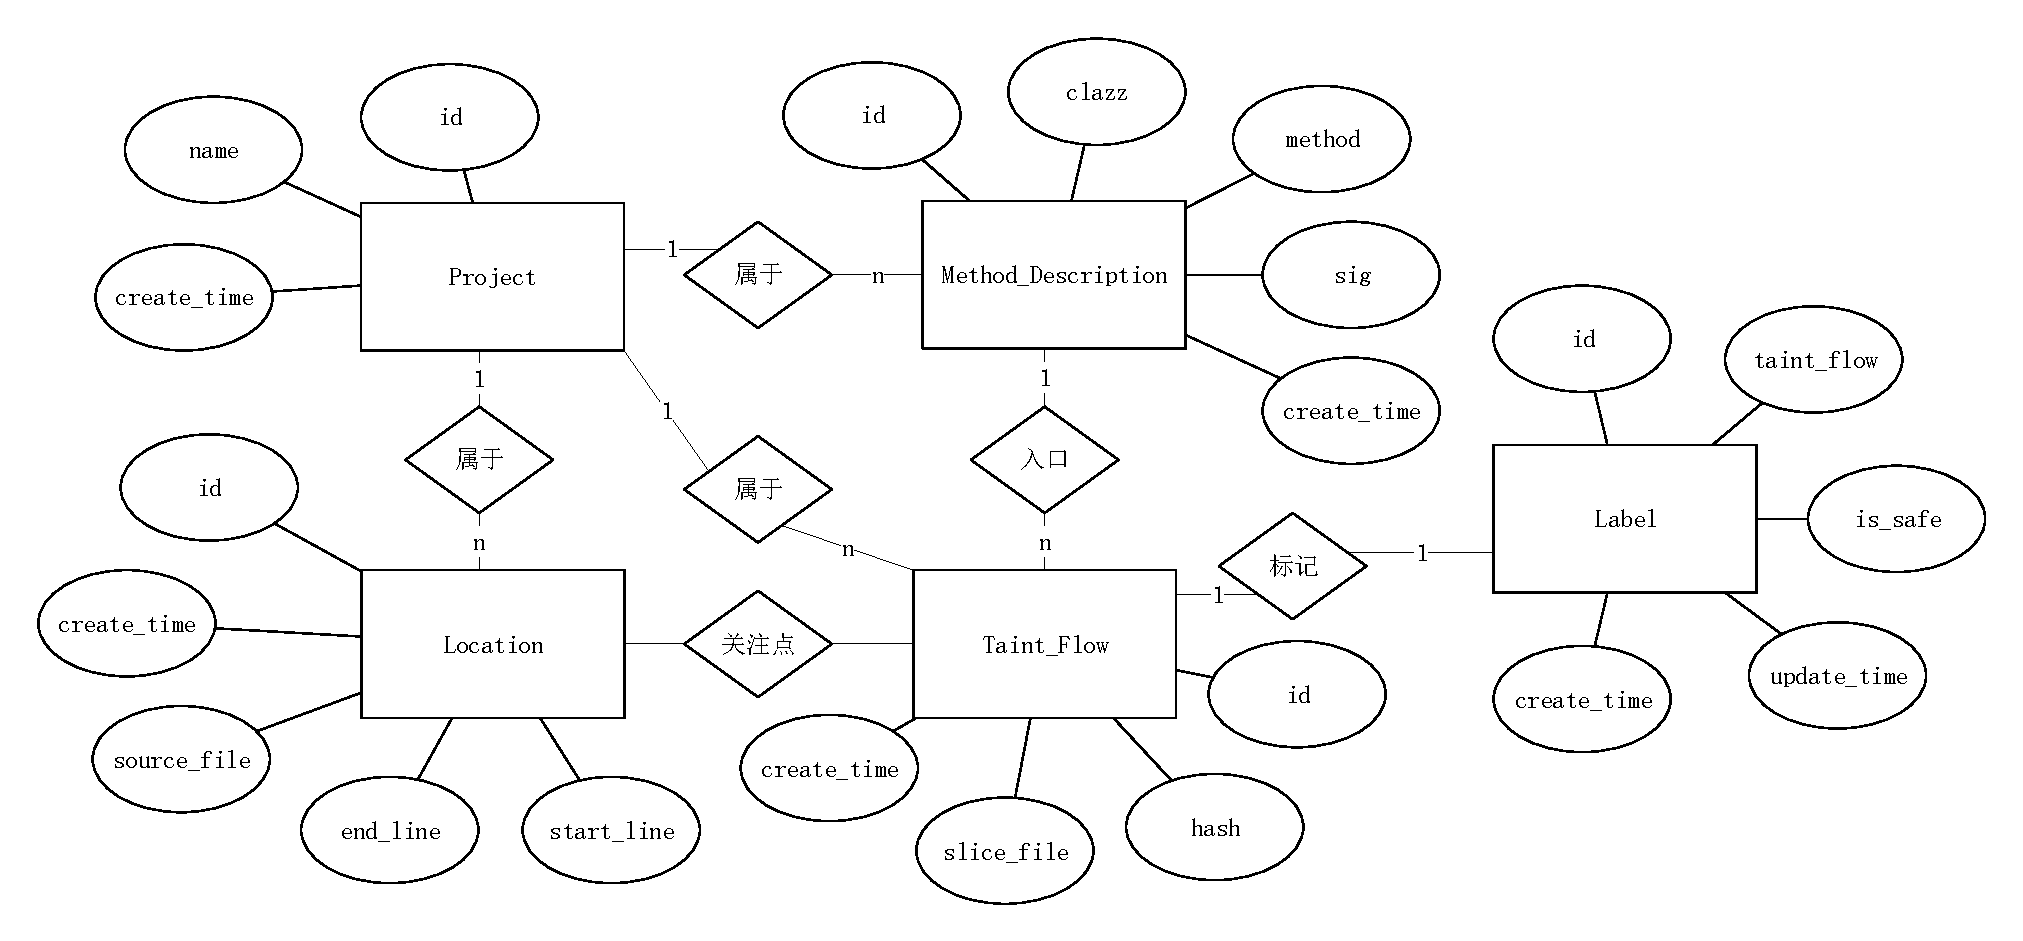
\includegraphics[width=1\linewidth]{FIGs/chapter3/program_er.pdf}
	\caption{与程序分析相关表的实体关系图}\label{er:program}
\end{figure}

表~\ref{sql:project}是对项目表的字段说明,其中,id是一个项目的唯一标识;name标识项目名称,存在唯一性约束,由客户端建立扫描项目时指定;create\_time记录该项目的创建时间。

\begin{table}[!htbp]\footnotesize %project table
	\centering
	\caption{Project 表}
	\vspace{2mm}
	% l - left, r - right, c - center. | means one vertical line 这里声明的是表格单元中的内容如何对齐
	\begin{tabular}{L{2cm}L{2cm}L{2.6cm}L{6cm}}
		\toprule
		\textbf{字段名}&\textbf{数据类型}&\textbf{属性}&\textbf{说明}\\
		\midrule
		id							&INT&PK&主键,项目的唯一标识\\
		name		 			&VARCHAR(255)&NN&表示项目的名称\\
		create\_time		  &DATETIME&NN&表示项目创建时间\\
		\bottomrule
	\end{tabular}
	\label{sql:project}
\end{table}

表~\ref{sql:methodDescription}是对函数摘要表的字段说明,其中,id 是一个函数摘要的唯一标识;clazz 记录函数的类名;method 记录函数的方法名;sig 记录函数签名,其包括了参数类型和返回值类型;project 作为外键,标识该函数摘要位于哪个项目中;create\_time记录该函数摘要的创建时间。此外,clazz,method,sig,project能够唯一标识一个函数摘要。
\begin{table}[!htbp]\footnotesize %methodDescription table
	\centering
	\caption{Method\_Description 表}
	\vspace{2mm}
	% l - left, r - right, c - center. | means one vertical line 这里声明的是表格单元中的内容如何对齐
	\begin{tabular}{L{2cm}L{2cm}L{2.6cm}L{6cm}}
		\toprule
		\textbf{字段名}&\textbf{数据类型}&\textbf{属性}&\textbf{说明}\\
		\midrule
		id					&INT&PK&主键,函数摘要的唯一标识\\
		clazz				&VARCHAR(255)&NN&表示该函数的类名\\
		method 			& VARCHAR(255) &NN&表示该函数的方法名\\
		sig					&VARCHAR(255)&NN&表示该函数的签名,即函数参数和返回值类型\\
		project  		  &INT&FK, NN&外键,指向Project,表示该函数出现在此项目中\\
		create\_time  &DATETIME&NN&表示标记创建时间\\
		\bottomrule
	\end{tabular}
	\label{sql:methodDescription}
\end{table}

表~\ref{sql:location}是对语句位置表的字段说明,其中,id是一个语句位置的唯一标识;source\_file记录该语句所在的文件名	;start\_line记录该位置开始的代码行号;end\_line记录该位置结束的代码行号  ;project作为外键,记录该位置位于哪个项目中;create\_time记录该项目的创建时间。此外,source\_file,start\_line,end\_line,project联合可以唯一标识一个语句位置。
\begin{table}[!htbp]\footnotesize %location table
	\centering
	\caption{Location 表}
	\vspace{2mm}
	% l - left, r - right, c - center. | means one vertical line 这里声明的是表格单元中的内容如何对齐
	\begin{tabular}{L{2cm}L{2cm}L{2.6cm}L{6cm}}
		\toprule
		\textbf{字段名}&\textbf{数据类型}&\textbf{属性}&\textbf{说明}\\
		\midrule
		id							&INT&PK&主键,语句位置的唯一标识\\
		source\_file		 	&VARCHAR(255)&NN&表示语句所在文件名\\
		start\_line 			& INT &NN, UNSIGNED&表示语句所在的开始行号\\
		end\_line				&INT&NN, UNSIGNED&表示语句所在的结束行号\\
		project  			  &INT&FK, NN&外键,指向Project,表示该位置出现在此项目中\\
		create\_time		  &DATETIME&NN&表示标记创建时间\\
		\bottomrule
	\end{tabular}
	\label{sql:location}
\end{table}

表~\ref{sql:taintFlow} 是对污染流表的字段说明,其中,id 是一个污染流的唯一标识;hash	是这个污染流的哈希,通过切片文本的SHA1得到;slice\_file 切片文件在硬盘上的保存位置,当数据库中记录删除时,切片文件也应被删除;entry和point分别为切片的入口点和关注点 ;project作为外键,记录污染流存在于哪个项目中;create\_time记录该污染流的创建时间。此外,entry,point和project可以联合唯一标识一个污染流记录。

\begin{table}[!htbp]\footnotesize %taintFlow table
	\centering
	\caption{Taint\_Flow 表}
	\vspace{2mm}
	% l - left, r - right, c - center. | means one vertical line 这里声明的是表格单元中的内容如何对齐
	\begin{tabular}{L{2cm}L{2cm}L{2.6cm}L{6cm}}
		\toprule
		\textbf{字段名}&\textbf{数据类型}&\textbf{属性}&\textbf{说明}\\
		\midrule
		id					&INT&PK&主键,污染流的唯一标识\\
		hash				&VARCHAR(255)&NN&表示污染流的哈希\\
	    slice\_file			& VARCHAR(255) &NN&表示污染流切片的文件名\\
		entry				&INT&FK&外键,指向Method\_Description,表示污染流切片的入口\\
		point				&INT&FK&外键,指向Location,表示污染流切片的结束位置\\
		project  		  &INT&FK, NN&外键,指向Project,表示污染流所在的项目\\
		create\_time  &DATETIME&NN&表示污染流的创建时间\\
		\bottomrule
	\end{tabular}
	\label{sql:taintFlow}
\end{table}

表~\ref{sql:label}是对标记表的字段说明,其中,id 是一个标记的唯一标识;taint\_flow 作为外键,指这被标记的污染流对象,同时一个污染流同时只能有一个标记;entry和point分别为切片的入口点和关注点 ;is\_safe 标记了该污染流是安全/不安全的;create\_time记录该标记的创建时间;update\_time记录该标记的更新时间。

\begin{table}[!htbp]\footnotesize %label table
	\centering
	\caption{Label 表}
	\vspace{2mm}
	% l - left, r - right, c - center. | means one vertical line 这里声明的是表格单元中的内容如何对齐
	\begin{tabular}{L{2cm}L{2cm}L{2.6cm}L{6cm}}
		\toprule
		\textbf{字段名}&\textbf{数据类型}&\textbf{属性}&\textbf{说明}\\
		\midrule
		id							&INT&PK&主键,标记的唯一标识\\
		taint\_flow		 		&INT &FK, NN&外键,指向Taint\_Flow,表示本标记的污染流对象\\
		is\_safe 				& BOOLEAN &NN&表示这个污染流是安全的\\
		create\_time		  &DATETIME&NN&表示标记创建时间\\
		update\_time		&DATETIME&NN&表示标记更新时间\\
		\bottomrule
	\end{tabular}
	\label{sql:label}
\end{table}

与模型相关的实体关系图如图~\ref{er:model} 所示,其中,模型配置(Model\_Config)表记录模型配置信息,主要包括了配置名,模型训练相关信息和 LSTM 模型的参数等,LSTM 模型表(LSTM\_Model)记录以训练好的模型信息,主要信息有训练度量,模型保存位置等,一个配置可以训练多个模型。

\begin{figure}[!htbp]
	\centering
	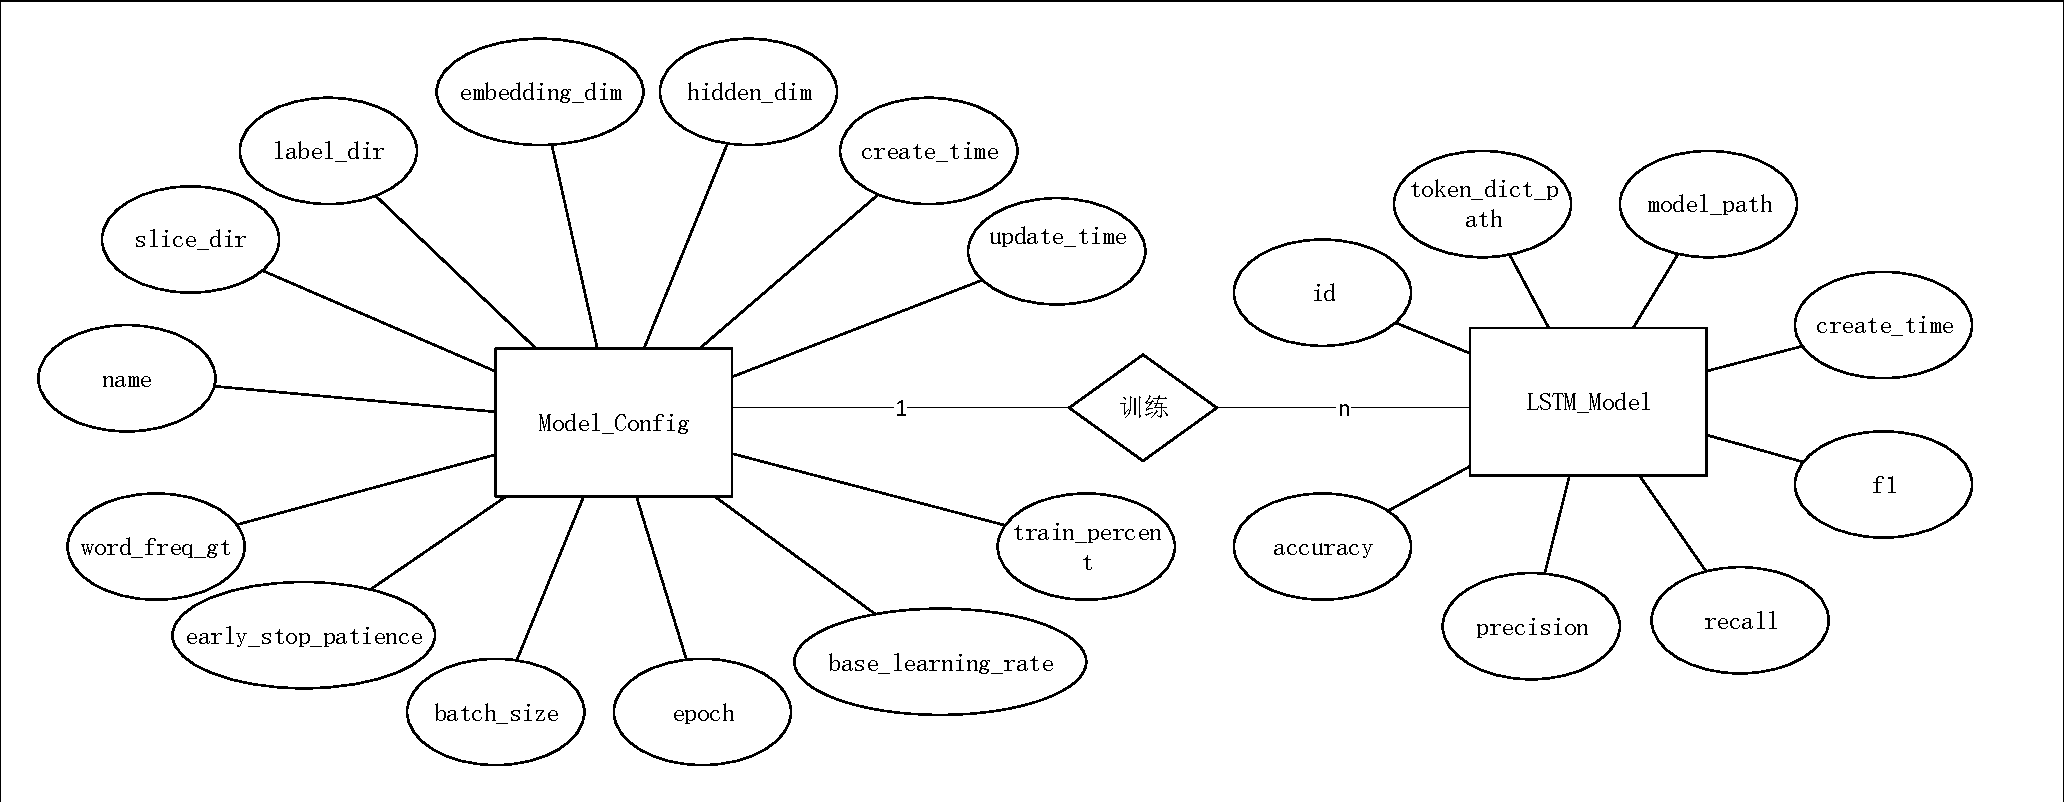
\includegraphics[width=1\linewidth]{FIGs/chapter3/model_er.pdf}
	\caption{与模型相关表的实体关系图}\label{er:model}
\end{figure}

 表~\ref{sql:modelConfigTable} 是对模型配置表的字段说明,其中 name 作为主键,用于唯一标识一个配置,训练时通过指定改值进行训练;slice\_dir 和 label\_dir 记录了学习用的数据集位置,分别表示了切片所在文件夹和标记所在文件夹(模型直接通过文件进行读取,而不从数据库读取,减少了IO消耗);embedding\_dim,hidden\_dim 为模型自身参数,分别代表词嵌入的维度和隐藏层神经元个数(模型的每层神经元个数相等);word\_freq\_gt 表示了将出现次数小于该值的单词表示为“UNK”(Unknown);early\_stop\_patience,base\_learning\_rate,batch\_size,epoch,train\_percent记录了模型训练的配置,early\_stop\_patience 值训练轮数超过改值后,若模型效果(loss)仍比之前最优效果差,则提前停止训练,base\_learning\_rate 指初始学习率,batch\_size 指批量传入模型的数据量,epoch 指最大训练轮数,train\_percent 指训练集占总数据集的百分比,剩下的数据作为训练集,用于评估训练效果;最后,create\_time 和 update\_time 分别表示配置创建时间和配置更新时间。

\begin{table}[!htbp]\footnotesize %model config table
	\centering
	\caption{Model\_Config 表}
	\vspace{2mm}
	% l - left, r - right, c - center. | means one vertical line 这里声明的是表格单元中的内容如何对齐
	\begin{tabular}{L{2.2cm}L{2cm}L{2.6cm}L{6cm}}
		\toprule
		\textbf{字段名}&\textbf{数据类型}&\textbf{属性}&\textbf{说明}\\
		\midrule
		name 						&VARCHAR(255)&PK&主键,唯一标识一个配置\\
		slice\_dir		 			&VARCHAR(255)&NN&模型使用切片数据所在的文件夹\\
		label\_dir		 			&VARCHAR(255)&NN&模型使用标记数据所在的文件夹\\
		embedding\_dim		  &INT&NN, UNSIGNED&词嵌入时的维度,值为正整数\\
		hidden\_dim				&INT&NN, UNSIGNED&隐藏层神经元的个数,值为正整数\\
		word\_freq\_gt			&INT&NN, UNSIGNED&最小词频,小于该词频则表示为UNK,值为正整数\\
		early\_stop\_patience		&INT&NN, UNSIGNED&提前停止忍耐度,如果学习轮数大于此值,效果仍比以前差则学习停止,值为正整数\\
		base\_learning\_rate		&DOUBLE&NN, UNSIGNED&初始学习率\\
		batch\_size					&INT&NN, UNSIGNED&批量数据记录数,每次向神经网络输入batch\_size条记录,再进行反向传播\\
		epoch						&INT&NN, UNSIGNED&训练最大迭代次数,超过该次数则停止训练\\
		train\_percent						&DOUBLE&NN, UNSIGNED&表示训练集占整个数据的百分比,默认为1,即将所有数据代入训练\\
		create\_time				&INT&NN, UNSIGNED&配置创建时间\\
		update\_time				&INT&NN, UNSIGNED&配置更新时间\\
		\bottomrule
	\end{tabular}
	\label{sql:modelConfigTable}
\end{table}

表~\ref{sql:lstmModelTable} 是对 BLSTM 模型表的字段说明,其中 id 作为主键唯一标识一个模型;token\_dict\_path 和 model\_path 分别表示单词到整形值的映射字典文件位置和BLSTM模型位置,这两个字段用于加载模型实现对切片的预测;config 表示模型是由何配置训练得到的;accuracy、precision、recall和F1表示了模型的四种度量,当配置划分没有训练集时,这些值为-1;create\_time记录模型被训练出的时间。

\begin{table}[!htbp]\footnotesize %lstm model table
	\centering
	\caption{BLSTM\_Model表}
	\vspace{2mm}
	% l - left, r - right, c - center. | means one vertical line 这里声明的是表格单元中的内容如何对齐
	\begin{tabular}{llll}
		\toprule
		\textbf{字段名}&\textbf{数据类型}&\textbf{属性}&\textbf{说明}\\
		\midrule
		id&INTEGER&PK&主键,模型的唯一标识\\
		token\_dict\_path &VARCHAR(255)&NN&保存单词到tokenid的字典文件位置\\
		model\_path		 &VARCHAR(255)&NN&保存BLSTM模型文件的位置\\
		config				 &VARCHAR(255)&FK,NN&指向Model\_Config表,表示模型对应的配置信息\\
		accuracy	&DOUBLE&NN&表示学习后训练集的准确率,若无训练集则为-1\\
		precision	&DOUBLE&NN&表示学习后训练集的精确率,若无训练集则为-1\\
		recall	&DOUBLE&NN&表示学习后训练集的召回率,若无训练集则为-1\\
		F1	&DOUBLE&NN&表示学习后训练集的F1,若无训练集则为-1\\
		create\_time		  &TIME&NN&记录模型创建时间\\
		\bottomrule
	\end{tabular}
	\label{sql:lstmModelTable}
\end{table}

\section{本章小结}